\section{Screw Theory}
\begin{frame}
	\frametitle{Lecture IV Outline}
	\begin{tcolorbox}[coltitle=yellow!50!black,colframe=magenta!25,split=.2,title=Lecture IV Outline]
		Screws Theory and Rigid Body Transformations.
		\tcblower
		Screws (properly revisited): Chasles' and Poinsot's theorem; Displacement and Force screws; Pl{\"u}cker coordinates.
		\vspace{.2cm}
		\newline
		Wrench; Instantaneous screw axis; Couple; Adjoint maps; Velocity transformations -- in Body and Spatial Homogeneous Coordinates.
		\vspace{.2cm}
		\newline
		Group theory: The Lie algebra, motions in $\mathfrak{se}(3)$;, and the Lie Group. 
		\vspace{.2cm}
		\newline
		Manipulator kinematics: Brockett's exponential map formula. Paden-Kahan subproblems.Denavit-Hartenberg Conventions.
	\end{tcolorbox}
\end{frame}

\begin{frame}
	\frametitle{Rigid Body Motions as Screws}
	%
	\begin{block}{Rigid Body Motion as a Screw Motion}
		The motion of a \textcolor{red}{rigid body} is precisely the same as if it were attached to  the \textcolor{red}{nut of a literal mechanical screw}. Associated with the screw is its pitch.
	\end{block}	
	%
	\begin{definition}[Screw]
		That straight line with which a \textcolor{red}{definite linear magnitude} termed the pitch is associated is called the \textcolor{red}{screw}.
	\end{definition}
\end{frame}


\begin{frame}
	\frametitle{Screw as a Geometric Quantity}	
	%	
	\begin{block}{Pitch of a Screw}
		\textcolor{brown}{The rectilinear distance}  through which (a literal nut)  \textcolor{red}{nut is translated parallel to the axis of a screw}, while the nut is rotated through the \textcolor{cyan}{angular unit of circular measure} is termed the \textcolor{light-blue}{pitch}.
	\end{block}
	%
	\begin{block}{Pl{\"u}cker Coordinates}
		Let \textcolor{red}{$\bm{a}$} be a point on line $\bm{\ell}_0$. Let \textcolor{red}{$\bm{a}$}'s direction cosine vector (to be introduced shortly) be \textcolor{red}{$\bm{b}$}. Then, its binormal (moment) vector is \textcolor{red}{$\bm{c=a\times b}$}. We say the pair \textcolor{red}{$(\bm{b},\bm{c})$} is the \textcolor{blue}{Pl{\"u}cker Coordinates} of point  \textcolor{red}{$\bm{a}$ on axis} $\bm{\ell}_0$.
	\end{block}	
\end{frame}

\begin{frame}
	\frametitle{Screw in Pl{\"u}cker Coordinates}
	%
	\begin{columns}[b]
		\begin{column}{.67\columnwidth}
			\centering
			\begin{definition}[Screw Coordinates]
				Six-vector, $\bm{s}$, related to the Pl{\"u}cker coordinates, parameterize a screw i.e. $\bm{s}=\left(s_1, s_2, s_3, s_4, s_5, s_6\right)$.
			\end{definition}
		\end{column}
		
		\begin{column}{.3\columnwidth}
			\centering
			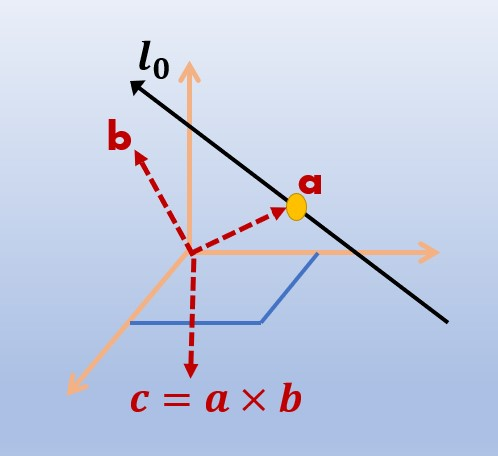
\includegraphics[width=\textwidth]{figures/plucker_coords.jpg}
		\end{column}
		\label{fig:plucker}
	\end{columns}
\end{frame}


\subsection{Displacement \& Twist}
\begin{frame}
	\frametitle{Screws and Pl{\"u}cker Coordinates}
	%
	\begin{block}{Screw axis and Pl{\"u}cker Coordinates}
		\begin{align}
			b_1 &= s_1, \quad b_2 = s_2, \quad b_3 = s_3; \\
			c_1 &= s_4 - p \cdot s_1, \quad c_2 = s_5-p\cdot s_2, \quad c_3 = s_6 - p\cdot s_3.
		\end{align}
	\end{block}
	%
	\begin{block}{Pitch in Pl{\"u}cker Coordinates}
		\begin{align}
			p &= \dfrac{s_1 \, s_4 + s_2 \, s_5 + s_3 \, s_6}{{s_1^2 + s_2^2 + s_3^2}}, \\
			\mid s \mid &= \sqrt{s_1^2 + s_2^2 + s_3^2} \quad \text{if } p \neq \infty, \\
			\mid s \mid &= \sqrt{s_4^2 + s_5^2 + s_6^2} \quad \text{if } p = \infty
		\end{align}
	\end{block}
\end{frame}


\begin{frame}
	\frametitle{Pitch and Magnitude of the screw}	
	\begin{block}{Pl{\"u}cker Coordinates' Direction Cosines}
		Suppose that 
		%\begin{align}
		$h = \sqrt{b_1^2+b_2^2+b_3^2}$.
		%\end{align}
		Then $(\bm{b}/h, \bm{c}/h)$ are respectively the direction cosines of the line, $l_0$ and its moment.
	\end{block}
	%
	\begin{block}{ Homogeneous Coordinates!}
		\textcolor{blue}{Pl{\"u}cker Coordinates} give six unit parameters of a point on a line. Pl{\"u}cker Coordinates are in \textcolor{red}{homogeneous coordinates}!
	\end{block}
\end{frame}

\begin{frame}
	\frametitle{Twist About a Screw (Axis)}
	%
	\begin{block}{Twist}
		A body's \textcolor{purple}{twist} about 
		s \textcolor{magenta}{screw} is a \textcolor{red}{uniform (infinitesimal) rotation} about the screw \textcolor{blue}{followed by a uniform (infinitesimal) translation} about an \textcolor{cyan}{axis parallel to the screw}, through \textcolor{magenta}{a distance that is the product of the pitch and the circular measure of rotation}.
	\end{block}	
	%
	\begin{block}{Twist}
		A \textcolor{purple}{twist} requires six 
		s \textcolor{magenta}{algebraic quantities} for its  \textcolor{red}{complete specification}:  \textcolor{blue}{five ($\{t_i\}_{i=1}^5$) specify the screw}, the \textcolor{cyan}{sixth (or its amplitude)} specifies the \textcolor{light-blue}{screw's rotaty angle}, $t_6$.
	\end{block}	
\end{frame}

\begin{frame}
	\frametitle{Twist in Pl{\"u}cker Coordinates}
	%
	\begin{definition}[Twist Coordinates]
		A six-vector, $\bm{t}$, related to the Pl{\"u}cker coordinates  parameterize a twist vector i.e. $\bm{t}=\left[(t_1, t_2, t_3), (t_4, t_5, t_6)\right]$ or $\bm{t}=\left(\bm{\omega}, \bm{v}\right)$, where $\bm{\omega}=(t_1, t_2, t_3)$ and $\bm{v}=(t_4, t_5, t_6)$.
	\end{definition}
	%
	\begin{block}{Pl{\"u}cker Coordinates of a Twist}
		\begin{align}
			b_1 &= t_1, \quad b_2 = t_2, \quad b_3 = t_3 \\
			c_1 &= t_4 - p \cdot s_1, \quad c_2 = t_5-p\cdot s_2, \quad c_3 = t_6 - p\cdot s_3.
		\end{align}
		%
	\end{block}
\end{frame}

\begin{frame}
	\frametitle{Twists in Pl{\"u}cker Coordinates}
	%
	\begin{block}{Pitch of the Twist}
		$p_t = \dfrac{t_1\,t_4 + t_2 \, t_5 + t_3\,t_6}{t_1^2+t_2^2+t_3^2}=\dfrac{\bm{\omega}\cdot \bm{v}}{\bm{\omega}\cdot \bm{\omega}}$.
	\end{block}
	%
	\begin{block}{Pitch of the Twist}
		Expressed as a ratio of the \textcolor{magenta}{magnitude of the velocity of a point on the twist axis} to the \textcolor{green}{magnitude of the angular velocity} about the twist axis. 
	\end{block}	
	%
	\begin{block}{Translation Distance}
		$d_t = t_6 \times p_t$.  The sign expresses the rotation's direction.
	\end{block}	
\end{frame}


\begin{frame}
	\frametitle{Twists and Fixed Movements}
	\begin{block}{Pure Rotation}
		Let pitch be \textcolor{light-blue}{zero}. That which results is but \textcolor{red}{pure rotation}.
	\end{block}
	
	\begin{block}{Pure Translation}
		Let pitch be \textcolor{magenta}{infinite}. That which results \textcolor{red}{cannot be a finite twist}, \textcolor{cyan}{except the amplitude be zero}, whereupon the \textcolor{brown}{twist becomes a pure translation parallel to the screw}.
	\end{block}
\end{frame}

%
\begin{frame}
	\frametitle{Curvilinear Displacement: Serret-Frenet Frame}
	\begin{columns}[]
		\begin{column}{.5\linewidth}
			\centering
			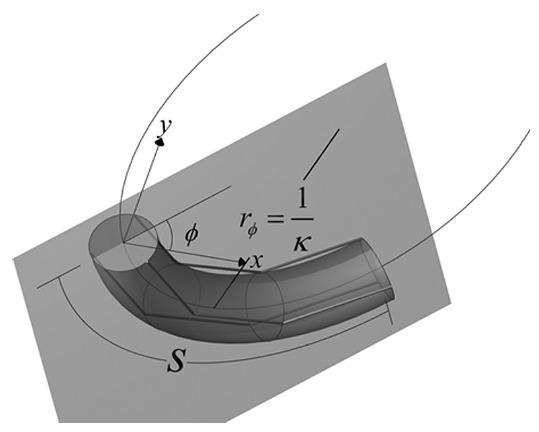
\includegraphics[width=\textwidth]{figures/multi_sec_manip.jpg}
		\end{column}
		\begin{column}{.68\linewidth}
			\centering
			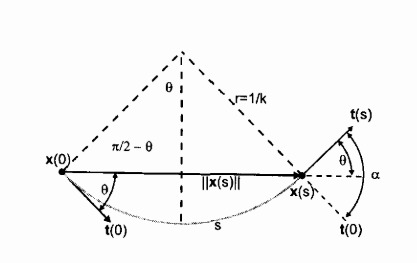
\includegraphics[width=\textwidth]{figures/serret.jpg}
		\end{column}
	\end{columns}
	\footnotesize{Elephant Trunk Multi-sectional Continuum Model (left), and its Representation in the Serret-Frenet Frame.}
\end{frame}
\begin{frame}
	\frametitle{Pl{\"u}cker Coordinates Example}
	\begin{block}{Chasles' Theorem Applied to The Serret-Frenet Frame}
		Consider a spatial curve $\bm{S}$ on the elephant continuum trunk shown earlier. Suppose $\bm{S}$ is parameterized by its arc length $\bm{s} \in [0, 1]$. 
		For a point $\bm{x}=\left[x, y, z\right]^T$ on $\bm{S}$, the unit tangent vector at $s$ is $\bm{t}(s)=\bm{dx}/\bm{ds}$.
	\end{block}
	%	
	\begin{block}{Differential Kinematics and The Serret-Frenet Frame}
		Denote by $\bm{n}$ the principal normal to $\bm{S}$ at $\bm{n}$; then we must have $\bm{b}=\bm{t}\times \bm{n}$ as the binormal. We say $(\bm{b},\bm{n})$ is the Pl{\"u}cker coordinate of the tangent $\bm{t}$.
	\end{block}
\end{frame}

\subsection{Force \& Wrench}
\begin{frame}
	\frametitle{Force}
	%	
	\begin{block}{Force}
		Net \textcolor{blue}{force} exerted on a body, 
		$\textcolor{red}{\bm{F}} = (f_x, f_y, f_z)$.
	\end{block}
	\begin{block}{Couple of Force}
		Suppose that $\bm{F}$ acts along a corkscrew axis. The resulting motion when $\bm{F}$ makes an infinitesimal rotation about its screw axis  is called its \textcolor{red}{couple}, $\mathfrak{C} = (c_x, c_y, c_z)$.
	\end{block}
	%	
\end{frame}

\begin{frame}
	\frametitle{Complete Wrench on a Screw}
	%	
	\begin{block}{Wrench}		
		A \textcolor{purple}{wrench} requires six 
		s \textcolor{magenta}{algebraic quantities} for its  \textcolor{red}{complete specification}:  \textcolor{blue}{five ($\{w_i\}_{i=1}^5$) specify the screw}, the \textcolor{cyan}{sixth (or its intensity)}, $w_6$, specifies the \textcolor{light-blue}{force's magnitude}.
	\end{block}
	%		
	\begin{block}{Couple's Moment}		
		The moment of the \textcolor{purple}{couple} is the product of the \textcolor{magenta}{intensity of the wrench} and the \textcolor{red}{ and the screw's pitch} i.e. $\alpha(\mathfrak{C}) = w_6 \times p_w$.
	\end{block}
	%	
\end{frame}

\begin{frame}
	\frametitle{Wrench on a Screw}
	%	
	\begin{block}{Wrench}
		Simple Definition: A \textcolor{brown}{force} and a \textcolor{cyan}{couple} both acting in a plane perpendicular to the force.
	\end{block}
	%
	\begin{definition}[Complete Definition]		
		The \textcolor{brown}{resultant canonical system of forces} acting on a rigid body, \textcolor{light-blue}{reduced to a resultant force on a point}, and acting along the \textcolor{red}{resultant couple} that is \textcolor{cyan}{perpendicular to the plane} in which the force acts is called \textcolor{blue}{the wrench}.
	\end{definition}
	%	
\end{frame}

\begin{frame}
	\frametitle{Wrench in Pl{\"u}cker Coordinates}
	%
	\begin{definition}[Wrench Coordinates]
		A six-vector, $\bm{w}$, related to the Pl{\"u}cker coordinates  parameterize a wrench vector i.e. $\bm{w}=\left[(w_1, w_2, w_3), (w_4, w_5, w_6)\right]$ or $\bm{w}=\left(\bm{f}, \bm{m}\right)$, where $\bm{f}=(w_1, w_2, w_3)$ and $\bm{m}=(w_4, w_5, w_6)$.
	\end{definition}
	%
	\begin{block}{Pl{\"u}cker Coordinates of a Wrench}
		\begin{align}
			b_1 &= w_1, \quad b_2 = w_2, \quad b_3 = w_3 \\
			c_1 &= w_4 - p \cdot s_1, \quad c_2 = w_5-p\cdot s_2, \quad c_3 = t_6 - p\cdot w_3.
		\end{align}
		%
	\end{block}
\end{frame}

\begin{frame}
	\frametitle{Wrench in Pl{\"u}cker Coordinates}
	%
	\begin{block}{Pitch of the Wrench}
		$p_t = \dfrac{w_1\,w_4 + w_2 \, w_5 + w_3\,w_6}{w_1^2+w_2^2+w_3^2}=\dfrac{\bm{f}\cdot \bm{m}}{\bm{f}\cdot \bm{f}}$.
	\end{block}
	%
	\begin{block}{Pitch of the Wrench}
		Expressed as a ratio of the \textcolor{magenta}{moment applied about a point on the axis} to the \textcolor{light-blue}{magnitude of the force applied}  along the wrench axis. 
	\end{block}	
	%
	\begin{block}{Wrench's Magnitude}
		$\|f\| = \sqrt{w_1^2 + w_2^2 + w_3^2}$ if $p_w = 0$ else $\|m\| = \sqrt{w_4^2 + w_5^2 + w_6^2}$ if $p_w = \infty$.
	\end{block}	
\end{frame}

\begin{frame}
	\frametitle{Wrenches and Fixed Movements}
	%	\begin{block}{Pitch of a Wrench, $p_w$}
		%		Acts along a (corkscrew) axis,  $p_w\bm{F}=\mathfrak{C}$.
		%	\end{block}
	%
	\begin{block}{Pure Force}
		Let pitch be \textcolor{light-blue}{zero}. That which results is \textcolor{red}{pure force} along its screw axis.
	\end{block}
	
	\begin{block}{Pure Couple}
		Let pitch be \textcolor{magenta}{infinite}. That which results \textcolor{red}{cannot be a finite wrench}, \textcolor{cyan}{except the intensity be zero}, whereupon the \textcolor{brown}{wrench becomes a pure couple in a plane that is perpendicular to the screw}.
	\end{block}
\end{frame}


\begin{frame}
	\frametitle{Statics and Instantaneous Kinematics}
	%
	\begin{block}{Statics and kinematics}
		\begin{center}
			\begin{tabular}{||c | c||} 
				\hline
				\textbf{Statics} & \textbf{Instantaneous Kinematics}  \\ %[0.5ex] 
				\hline\hline
				Force,  $\bm{F}$ about $n$. & Infinitesimal rotation, $\bm{\omega}$ \\ 
				\hline
				Couple, $\mathfrak{C}$: [$\bm{F}$] $\times$ [$\ell$] & Infinitesimal translation, $\bm{t}$ \\
				\hline
				$p_w = \pm \mathfrak{C}/\bm{F}$ & Pitch of a Wrench, $\bm{w}$ \\
				\hline
				$\mid\bm{F} \mid$ & Intensity of Wrench \\
				\hline
			\end{tabular}
			\text{Dyname}: $(\bm{F}, \mathfrak{C})$. Credits: Pl{\"u}cker (1866), Routh (1892).
		\end{center}
	\end{block}
	
\end{frame}

\subsection{Screws in Pl{\"u}cker Coordinates}
\begin{frame}
	\frametitle{Pl{\"u}cker Coordinates Kinetics Quiz}
	%
	\begin{block}{Poinsot's Theorem Quiz on a  Force and its Moment}
		Suppose that a force $\bm{F}$  acts at the point $\bm{a}$ in the image of Frame \ref{fig:plucker}. What are the Pl{\"u}cker coordinates of the \textcolor{red}{line of force}?
	\end{block}
\end{frame}

\note{
	\begin{frame}
		%
		\begin{block}{Poinsot's Theorem Quiz on a  Force and its Moment}
			Imagine that a force $\bm{F}$ is acting at the point $\bm{a}$ in the image of Frame \ref{fig:plucker}. Suppose that $\bm{\tau}$ is torque acting along the normal to point $\bm{a}$.  Then $(\bm{f,\tau})$ are the Pl{\"u}cker  coordinates of the \textcolor{red}{line of force}.
		\end{block}
		%
		\begin{block}{Arithmetics on Screws}
			Scalar and vector arithmetic operations are valid on infinitesimal  screws e.g.
			\begin{align}
				c_1 \bm{s}_1 + c_2 \bm{s}_2 = 0 \text{ for } c_1, \, c_2 \neq 0 \text{ on screws } \bm{s}_1, \bm{s}_2.
			\end{align}
		\end{block}
	\end{frame}
}


\begin{frame}
	\frametitle{Pl{\"u}cker Coordinates Kinetics Quiz}
	%
	\begin{block}{Poinsot's Theorem Quiz on a  Force and its Moment}
		Suppose that a force $\bm{F}$  acts at the point $\bm{a}$ in the image of Frame \ref{fig:plucker}. What are the Pl{\"u}cker coordinates of the \textcolor{red}{line of force}?
	\end{block}
\end{frame}


\subsection{Group Theory Connections}
\begin{frame}
	\frametitle{Group Theory Review}
	\begin{block}{The Euclidean Motion}
		Let $\mathbb{E}^3$ denote the ordinary Cartesian 3-space that admits the standard inner product 
		%
		\begin{align}
			\langle x, y \rangle = \sum_i x_i \, y_i.
		\end{align}
	\end{block}

	\begin{block}{Transformations}
		The set of all \textcolor{brown}{length-preserving transformations} in $\mathbb{E}^3$ shall be denoted by $\mathbb{E}(3) \in \mathbb{R}^6$ \ie the family of \textcolor{cyan}{translations and rotations}\footnote{Rotations in $\mathbb{E}^3$ are not necessarily proper.}.
	\end{block}
\end{frame}


\begin{frame}
	\frametitle{Group Transformation Isomorphism}
	\begin{block}{Brockett, 1990}
		\textcolor{brown}{Euclidean transformation under group composition} and  \textcolor{cyan}{Euclidean transformation under group multiplication} preserve the \textcolor{red}{isomorphic property}.
	\end{block}
	
	\begin{block}{Example: Affine Euclidean Transformations}
		$\bm{q}$ defines a \textcolor{brown}{Euclidean} \textcolor{light-blue}{affine transformation} $\bm{q} = \rot \bm{x} + \bm{d}$ \text{ if } $\langle \rot, \rot^T\rangle = \identity$ for $(\bm{q}, \bm{d}) \in \reline^3$. Now, suppose $\bm{q} = \rot_1 \bm{x} + \bm{d}_1$ and $\bm{p} = \rot_2 \bm{q} + \bm{d}_2$, then $\bm{p} = \rot_2 \rot_1\bm{x}+ \bm{d}_2$. %and $\bm{p} = \rot_2 \bm{q} + \bm{d}_2$
	\end{block}
\end{frame}


\begin{frame}
	\frametitle{Group Transformation Isomorphism}
	\begin{block}{Example: Euclidean Transformation Identity}
		\begin{align}
			\left(
			\begin{array}{cc}
				\rot_2 & \bm{d}_2 \\
				0 & 1
			\end{array}
			\right)
			\left(
			\begin{array}{cc}
				\rot_1 & \bm{d}_1 \\
				0 & 1
			\end{array}
			\right) = 
			\left(
			\begin{array}{cc}
				\rot_2 \rot_1 & \rot_2\bm{d}_1 + \bm{d}_2 \\
				0 & 1
			\end{array}
			\right)
		\end{align}
	\end{block}

	\begin{block}{The isomorphic property (Brockett, 1990)}
		That matrices of the form (SE(3) matrices):
		%\begin{align}
		$	\left(
			\begin{array}{cc}
				\rot & \bm{d} \\
				0 & 1
			\end{array}
			\right) $
		%\end{align}
	are isomorphic.
	\end{block}
\end{frame}

\begin{frame}
	\frametitle{The General Linear Group}
	\begin{block}{$SO(3)$ as a General Linear Group}
		The \textcolor{brown}{special orthogonal group, $\orthoggroup$,} is a \textcolor{blue}{subgroup} of the \textcolor{magenta}{general linear group}
		%
		\begin{align}
			\orthoggroup = \{\rot \in GL(n, \mathbb{R}): \rot \, \rot^T = \identity, \text{det } \rot = \identity \}.
		\end{align}
	\end{block}
\end{frame}

\begin{frame}
	\frametitle{The Lie Group}
	
	\begin{block}{The Lie Group}
		A group with a \textcolor{brown}{topology operation on its set of elements} such that the group can be given the \textcolor{blue}{structure of a differential manifold} with the property that \textcolor{magenta}{group multiplication and inversion} is \textcolor{blue}{continuous} is called a \textcolor{brown}{Lie group}.
	\end{block}
	
	\begin{block}{The Special Euclidean Matrix Group, $\liegroup(3)$}
		$\liegroup(3)$ is a \textcolor{brown}{differentiable manifold}, comprised of all the \textcolor{cyan}{translations} and \textcolor{blue}{proper rotations} that \textcolor{red}{moves a body from one point to another} in the ordinary cartesian 3-space $\textbf{E}^3$.
	\end{block}
\end{frame}

\begin{frame}
	\frametitle{The Lie Group}	
	\begin{block}{The Special Euclidean Matrix Group, $\liegroup(3)$}
		\begin{align}
			g = \begin{bmatrix}
				\bm{R} & \bm{d} \\ \bm{0}^T & 1
			\end{bmatrix}; g \in \liegroup(3).
			\label{eq:rigid_trans}
		\end{align}
	\end{block}
\end{frame}

\begin{frame}
	\frametitle{The Lie Group}	
	\begin{block}{The Special Euclidean Matrix Group, $\liegroup(3)$}
		\begin{align}
			\liegroup(3) = \{(\rot, d): \rot \in \orthoggroup, d \in \reline^3 \}:=\orthoggroup \times \reline^3.
			\label{eq:se3_rep}
		\end{align}
		 \footnotesize{I have followed \textcolor{brown}{Chasles' notation}, who posited that \textcolor{cyan}{any rigid motion can be formed via a rotation}, \textcolor{brown}{followed by a translation}, and that \textcolor{purple}{the rotation and the translation commute} i.e. $\rot \, d = d$}.
	\end{block}

	\begin{block}{The Special Euclidean Matrix Group, $\liegroup(3)$}
		\footnotesize{Note: Most authors' notation follow \textcolor{red}{Euclid's theorem} i.e. any rigid motion is a \textcolor{magenta}{translation} followed by a \textcolor{cyan}{rotation about an axis} that \textcolor{blue}{passes through a pre-specified (fixed) point}.}	
		\begin{align}
			\liegroup(3) = \{(d, \rot):  d \in \reline^3, \rot \in \orthoggroup 	\}:=  \reline^3 \times \orthoggroup.
			\label{eq:se3_rep_euclid}
		\end{align}
	\end{block}
\end{frame}

\begin{frame}
	\frametitle{The Lie Group}		
	\begin{block}{The Special Euclidean Matrix Group, $\liegroup(3)$}
		\textcolor{blue}{Chasles' notation} allows for \textcolor{purple}{motion representation} in form of \textcolor{red}{screw motions}.
	\end{block}
	
	\begin{block}{Commutativity of group operations on $\liegroup(3)$}
		\textcolor{cyan}{[Brockett, 1990]}: Equation \eqref{eq:se3_rep} %and \eqref{eq:se3_rep_euclid} 
		imply that the \textcolor{blue}{Lie group} is a \textcolor{magenta}{semidirect product of simple Lie subgroup of orthogonal transformations} and the \textcolor{red}{abelian Lie subgroup of all translations}.
	\end{block}
\end{frame}



\begin{frame}
	\frametitle{The Lie Algebra}	
	\begin{block}{The Lie Algebra, $\liealg(3)$}
		The \textcolor{cyan}{Lie algebra} is a \textcolor{brown}{vector space} $\hat{\bm{\xi}} $ with the \textcolor{magenta}{antisymmetric bilinear operation} $[,]: \hat{\bm{\xi}}  \times \hat{\bm{\xi}} \rightarrow \hat{\bm{\xi}} $ which satisfies the \textcolor{cyan}{Jacobi identity}, 
		\begin{align}
			[\hat{\bm{\xi}}_1, [\hat{\bm{\xi}}_2, \hat{\bm{\xi}}_3]] +[\hat{\bm{\xi}}_2, [\hat{\bm{\xi}}_3, \hat{\bm{\xi}}_1]] + [\hat{\bm{\xi}}_3, [\hat{\bm{\xi}}_1, \hat{\bm{\xi}}_2]] = 0.
		\end{align}
		\footnotesize{NB: $[,]$ is alternatively the \textcolor{blue}{Lie bracket notation with antisymmetry operation $[\hat{\bm{\xi}}_2, \hat{\bm{\xi}}_3] = -[\hat{\bm{\xi}}_3, \hat{\bm{\xi}}_2]$}.}
	\end{block}
\end{frame}


\begin{frame}
	\frametitle{The Lie Algebra Representation}	
	\begin{block}{The Lie Algebra Representation, $\liealg(3)$}
		The \textcolor{cyan}{Lie algebra} admits the following \textcolor{red}{homogeneous coordinates representation} for a point $q \in \reline^3$ on a \textcolor{magenta}{link that rotates with unit velocity $\omega$}, 
		\begin{align}
			\hat{\bm{\xi}} =  \left(\begin{array}{cc}
				\tilde{\omega} & v \\
				0 & 0
			\end{array}\right) \in \liealg(3), \,\bm{\xi}=\left(\omega^T, v^T\right)^T \in \reline^6
		\end{align}
		{where $v = -\omega \times q$.}
	\end{block}
\end{frame}

\begin{frame}
	\frametitle{The Lie Algebra Representation}	
	\begin{block}{The Lie Algebra Representation, $\liealg(3)$}
		Observe:  
		\begin{align}
			\tilde{\omega} =  \left(\begin{array}{ccc}
				0 & -\omega_z & \omega_y \\
				\omega_z & 0 & -\omega_x \\
				-\omega_y &  \omega_x & 0
			\end{array}\right) \equiv -\tilde{\omega}^T \in \mathfrak{so}(3)
		\end{align}
		{is the \textcolor{red}{skew-symmetric form of the velocity of the tip point}, $\omega \in \reline^3$.}
	\end{block}
\end{frame}

\begin{frame}
	\frametitle{The Lie Algebra Diffeomorphisms}	
	\begin{block}{Lie Representation Snippet}
		Observe:  
		\begin{align}
			\tilde{(\cdot)}_{SO(3)}: &\reline^3 \rightarrow \mathfrak{so}(3) \\
			\tilde{(\cdot)}_{SE(3)}: &\reline^6 \rightarrow \mathfrak{se}(3) 
		\end{align}
		$\tilde{\omega}(S)\in \liealg(3)$: e.g. \textcolor{blue}{Twist parameterization} of a curve, deformation, \textcolor{red}{screw}.
		
		${\omega}(S)\in \reline^6$: e.g. \textcolor{blue}{Motion vector} e.g. linear + angular velocities, axial, shear, bending, and torsion motion.
	\end{block}
\end{frame}


\begin{frame}
	\frametitle{The exponential map belongs to the Lie Group}	
	\begin{block}{The exponential map, $exp(\mathfrak{se}(3))$, is an element of $SE(3)$}
		Given $g:  \left(\begin{array}{cc}
			\rot(\theta) & \bm{d} \\
			0 & 1
		\end{array}\right) \in SE(3)$ there exists a $\tilde{\bm{\xi}}=(\tilde{\omega}, v) \in \mathfrak{se}(3)$, such that  $exp(\tilde{\bm{\xi}} \theta) \in SE(3)$\footnote{Proof in Murray and Sastry, Prop 2.8.}.
	\end{block}
	
	\begin{block}{The exponential map, $exp(\mathfrak{se}(3))$, is surjective onto $SE(3)$}
		Given $g:  \left(\begin{array}{cc}
			\rot(\theta) & \bm{d} \\
			0 & 1
		\end{array}\right) \in SE(3)$ there exists a $\left(\begin{array}{cc}
		\tilde{\omega} & \bm{d} \\
		0 & 0
	\end{array}\right); \tilde{\omega}=-\tilde{\omega}^T$, such that  $exp(\tilde{\omega}) =g$\footnote{Proof in Murray and Sastry, Prop 2.9.}.
	\end{block}
\end{frame}

\begin{frame}
	\frametitle{Chasles and Affine Transformations}	
	\begin{block}{Chasles Theorem and Affine Transformations}
		\begin{align}
			\left(
			\begin{array}{cc}
				\rot & \bm{d} \\
				0 & 1
			\end{array}
			\right) = \left(
			\begin{array}{cc}
				\identity & \bm{c} \\
				0 & 1
			\end{array}
			\right)
			%
			\left(
			\begin{array}{cc}
				\rot & \bm{d} \\
				0 & 1
			\end{array}
			\right)
		\end{align}
		with $\rot\, \bm{d}=\bm{d}$. Note $\langle \bm{c}, \bm{d}\rangle=0$ for $\bm{c}$ and $\bm{d}$ to be unique.
	\end{block}
\end{frame}


\begin{frame}
	\frametitle{Screm Motion and Exponential Map}	
	\begin{block}{Screw Motion and Exponential Map (Brockett, 1990)}
		Range and null space of a $\tilde{\omega}$ are orthogonal. Thus,
		%
		\begin{align}
			\left(\begin{array}{cc}
				\identity & \bm{c} \\
				0 & 1
			\end{array}\right)
			%			
			\left(\begin{array}{cc}
				\tilde{\omega} & \bm{d} \\
				0 & 0
			\end{array}\right)
			%			
			\left(\begin{array}{cc}
					\identity & -\bm{c} \\
					0 & 1
			\end{array}\right) = 
			%			
			\left(\begin{array}{cc}
				\tilde{\omega} & \bm{d}-\tilde{\omega}\bm{c} \\
				0 & 0
			\end{array}\right)
		\end{align}
		 establishes that every motion of the form $\left(\begin{array}{cc}
		 	\tilde{\omega} & \bm{d} \\
		 	0 & 0
		 \end{array}\right)\theta$ is a \textcolor{red}{screw motion w.r.t some origin}.
	\end{block}
\end{frame}


\begin{frame}
	\frametitle{Group Composition and Screws Connection}	
	\begin{block}{The Lie Algebra Representation, $\liealg(3)$}
		Observe:  
		\begin{align}
			\tilde{(\cdot)}_{SO(3)}: &\reline^3 \rightarrow \mathfrak{so}(3) \\
			\tilde{(\cdot)}_{SE(3)}: &\reline^6 \rightarrow \mathfrak{se}(3) 
		\end{align}
		$\tilde{\omega}(S)\in \liealg(3)$: \textcolor{blue}{Twist parameterization} of a curve, deformation, \textcolor{red}{screw}.
		
		${\omega}(S)\in \reline^6$: \textcolor{blue}{Motion vector} e.g. linear + angular velocities, axial, shear, bending, and torsion motion.
	\end{block}
\end{frame}